% Povinný argument: Kód předmětu
\newcommand{\subject}{BPC-DAK}
% Povinný argument: Název předmětu
\newcommand{\subjectname}{Datová komunikace}
% Povinný argument: Seznam autorů
\newcommand{\authors}{On}
% Povinný argument: Seznam korektorů
\newcommand{\corrections}{Já}
% Nepovinný argument: Popis dokumentu
\newcommand{\docdesc}{Otázky ke zkoušce}
% Nepovinný argument: Cílová skupina dokumentu
\newcommand{\docgroup}{Informační bezpečnost, FEKT VUT}
% Nepovinný argument: URL repozitáře nebo jiný odkaz na dokument
\newcommand{\docurl}{https://github.com/VUT-FEKT-IBE/FEKT.tex}

% Přepsáním argumentu na 'false' vypnete balíček 'minted' pro sázení kódu.
% Pro jeho použití lokálně musíte mít v systému dostupný Python 3, python
% knihovnu 'minted' a PDFLaTeX musíte spouštět s argumentem '-shell-escape'.
% Místo něj můžete použít prostředí 'lstlisting'.
\newcommand{\docminted}{true}

% FEKT.tex
% https://github.com/VUT-FEKT-IBE/FEKT.tex
% Git hash repozitáře v době kopírování:

\documentclass[
    % Velikost základního písma je 12 bodů
    12pt,
    % Formát papíru je A4
    a4paper,
    % Oboustranný tisk
    oneside,
    % Záložky a metainformace ve výsledném PDF budou v kódování unicode
    unicode,
]{article}

%%%%%%%%%%%%%%%%%%%%
% OBECNÉ NASTAVENÍ %
%%%%%%%%%%%%%%%%%%%%

% Kódování zdrojových souborů
\usepackage[utf8]{inputenc}
% Kódování výstupního souboru
\usepackage[T1]{fontenc}
% Podpora češtiny
\usepackage[czech]{babel}

% Geometrie stránky
\usepackage[
    % Horní a dolní okraj
    tmargin=25mm,
    bmargin=25mm,
    % Vnitřní a vnější okraj
    lmargin=30mm,
    rmargin=20mm,
    % Velikost zápatí
    footskip=17mm,
    % Vypnutí záhlaví
    nohead,
]{geometry}

% Zajištění kopírovatelnosti a prohledávanosti vytvořených PDF
\usepackage{cmap}
% Podmínky (pro použití v titulní straně)
\usepackage{ifthen}

%%%%%%%%%%%%%%%
% FORMÁTOVÁNÍ %
%%%%%%%%%%%%%%%

% Nastavení stylu nadpisů
\usepackage{sectsty}
% Formátování obsahů
\usepackage{tocloft}
\setcounter{tocdepth}{1}
% Odstranění mezer mezi řádky v seznamech
\usepackage{enumitem}
\setlist{nosep}
\setitemize{leftmargin=1em}
\setenumerate{leftmargin=1.5em}
\renewcommand{\labelitemi}{--}
\renewcommand{\labelitemii}{--}
\renewcommand{\labelitemiii}{--}
\renewcommand{\labelitemiv}{--}
% Sázení správných uvozovek pomocí '\enquote{}'
\usepackage{csquotes}
% Vynucení umístění poznámek pod čarou vespod stránky
\usepackage[bottom]{footmisc}
% Automatické zarovnání textu k předcházení vdov a parchantů
\usepackage[defaultlines=3,all=true]{nowidow}
% Zalomení části textu pokud není na současné stránce dost místa
\usepackage{needspace}
% Nastavení řádkování
\usepackage{setspace}
\onehalfspacing
% Změna odsazení odstavců
\setlength{\parskip}{1em}
\setlength{\parindent}{0em}

% Bezpatkové sázení nadpisů
\allsectionsfont{\sffamily}
% Změna formátování nadpisu a podnadpisů v Obsahu
\renewcommand{\cfttoctitlefont}{\Large\bfseries\sffamily}
\renewcommand{\cftsubsecdotsep}{\cftdotsep}

% Použití moderní/aktualizované sady písem
\usepackage{lmodern}

%%%%%%%%%%%
% NADPISY %
%%%%%%%%%%%

\usepackage{titlesec}

\titlespacing*{\section}{0pt}{10pt}{-0.2\baselineskip}
\titlespacing*{\subsection}{0pt}{0.2\baselineskip}{-0.2\baselineskip}
\titlespacing*{\subsubsection}{0pt}{0.2\baselineskip}{-0.2\baselineskip}
\titlespacing*{\paragraph}{0pt}{0pt}{1em}

%%%%%%%%%%
% ODKAZY %
%%%%%%%%%%

% Tvorba hypertextových odkazů
\usepackage[
    breaklinks=true,
    hypertexnames=false,
]{hyperref}
% Nastavení barvení odkazů
\hypersetup{
    colorlinks,
    citecolor=black,
    filecolor=black,
    linkcolor=black,
    urlcolor=blue
}

%%%%%%%%%%%%%%%%%%%%%%%%%%%
% OBRÁZKY, GRAFY, TABULKY %
%%%%%%%%%%%%%%%%%%%%%%%%%%%

% Vkládání obrázků
\usepackage{graphicx}
\usepackage{subfig}
% Nastavení popisů obrázků, výpisů a tabulek
\usepackage{caption}
\captionsetup{justification=centering}
% Grafy a vektorové obrázky
\usepackage{tikz}
\usetikzlibrary{shapes,arrows}
% Složitější tabulky
\usepackage{tabularx}
\usepackage{multicol}

% Sázení osamocených float prostředí v horní části stránky
\makeatletter
\setlength{\@fptop}{0pt plus 10pt minus 0pt}
\makeatother

% Vynucení vypsání floating prostředí pomocí \FloatBarrier
\usepackage{placeins}

%%%%%%%%%%%%%%
% MATEMATIKA %
%%%%%%%%%%%%%%

% Sázení matematiky a matematických symbolů ('\mathbb{}')
\usepackage{amsmath}
\usepackage{amssymb}
% Sázení fyzikálních veličin
\usepackage{siunitx}

%%%%%%%%%%%%%%%%%
% ZDROJOVÉ KÓDY %
%%%%%%%%%%%%%%%%%

% Sazba zdrojových kódů
\usepackage[formats]{listings}
% Přepnutí prostředí 'code' do režimu výpisu kódu
\newenvironment{code}{\captionsetup{type=listing}}{}

\lstset{
    basicstyle=\small\ttfamily,
    numbers=left,
    numberstyle=\tiny,
    tabsize=4,
    columns=fixed,
    showstringspaces=false,
    showtabs=false,
    keepspaces,
}

% Balíček 'minted' budeme používat pouze pokud je jeho hodnota nastavena na 'true'
\providecommand{\docminted}{false}
\ifthenelse{\equal{\docminted}{true}}
{
    % Sazba zdrojových kódů
    \usepackage[newfloat]{minted}
    % Nastavení barev 'minted' kódů
    \usemintedstyle{pastie}
}
{
    % \docminted není 'true', nic neprovádíme
    % Pokud je v dokumentu 'minted' prostředí, dokument se nepodaří přeložit.
}

%%%%%%%%%%%
% TITULKA %
%%%%%%%%%%%

\IfFileExists{./.repo.tex}{
    % Soubor '.repo.tex' může (re)definovat povinné a nepovinné argumenty
    % souboru 'main.tex'. To lze využít v případech kdy v jednom repozitáři
    % existuje více dokumentů najednou (např. státnicové otázky).
    \input{.repo}
}{}

% Pokud byly nepovinné argumenty zakomentovány nebo vymazány, přidáme prázdné
% definice příkazů, aby bylo dokument možné správně přeložit.
\providecommand{\docdesc}{}
\providecommand{\docgroup}{}
\providecommand{\docurl}{}

\newcommand{\titulka}{
    \vspace*{2em}
    \begin{center}
        {\Huge \bfseries \subject}

        \vspace*{1em}

        {\Huge \bfseries \subjectname}

        \vspace*{2em}

        {\Large \docdesc}

        \vspace*{1em}

        \docgroup

        \url{\docurl}
    \end{center}

    \vfill

    \begin{tabular}{ll}
        Text:      & \authors     \\
        Korektura: & \corrections \\
    \end{tabular}
    \hfill
    \today

    \thispagestyle{empty}
    \newpage
}

\usepackage{mdframed}

\begin{document}

\titulka{}

\tableofcontents
\thispagestyle{empty}

\setcounter{page}{0}

\clearpage
\section{Základní poznatky z teorie informace}
\subsection{Vysvětlete pojmy množství informace a entropie}
\begin{itemize}
    \item \textbf{Množství informace} = I
    \begin{itemize}
        \item Jde o množství informace, které nese  každá jednotlivá zpráva S$_i$
        \item Jednotkou je Shannon (Sh)
    \end{itemize}
    \item \textbf{Entropie} 
    \begin{itemize}
        \item Průměrné množství informace nesené jednou zprávou
    \end{itemize}
    \item \textbf{Entropie zdroje} = H
    \begin{itemize}
        \item Průměrné množsví informace na jeden symbol
        \item Jednotka je Sh/symbol
    \end{itemize}
\end{itemize}

\subsection{ Vysvětlete rozdíl mezi jednotkami Shannon a bit}
\begin{itemize}
    \item Shannon je jednotka informace
    \item Bit je jednotka dat
    \item data != informace
\end{itemize}

\subsection{3.	Vysvětlete pojem základní zdroj zpráv, čím je určen a jaké jsou jeho vlastnosti}
Jedná se o diskrétní prvek, jelikož k popisu je oizžut jibečbž oičet charakteristických prvků.
Je určen množinou zpráv S = ${S_i}$´, kde každá s$_i$ je generována zdrojem s pravděpodobností p, přičemž platí, že $\sum p_i = 1$.
Množinu S nazýváme také abeceda zdroje, jednotlivé zprávy jsou symboly.

\subsection{Co je to nadbytečnost zdroje }
\textbf{Nadbytečnost} = R.
Jinak také \textit{redundance}.
R nabývá hodnot 0-1.
Vhodným kódováním a kompresí se snažíme snížit její hodnotu k 0.

\subsection{Vysvětlete pojem přizpůsobený zdroj zpráv a zdrojové kódovaní}
Používá se v praxi, kdy je potřeba přizpůsobit základní zdroj pro potřeby přenosu přenosovým kanálem.
Důvodem je nedostate k sigálových stavů vzhledem k počtu symbolů základního zdroje. Přízpůsobením zdroje na další přenost je použit pomocný zdroj, který má definován vyhovující počet symbolů. Pomocný zdroj je určen množinou X = ${x_i}$.
Zdrojové kódování jako přiřazení $s_i => x_i,x_s,x_k$\dots pro každý prvek abecedy X, hovoříme tedy o n-násobně rozšířeném zdroji informace. Zdrojové kódování se dále dělí na rovnoměrné (všechny značky stejné dlouhé, n=konst) a nerovnoměrné (značky jsou různých délek.

\subsection{Vysvětlete pojem účinnost kódování pro rovnoměrné a nerovnoměrné kódování}
Účinnost kódování je ekvivalentem entropie základního zdroje a je vyšší při použití nerovnoměrného kódování.

\subsection{7.	Jaké jsou statistické a dynamické charakteristiky přizpůsobeného zdroje zpráv}
\textbf{Statistické}
\begin{itemize}
    \item Entropie přizpůsobeného zdroje
    \item Max entropie přizpůsobeného zddroje
    \item Účinnost kódování
    \item Redundance přizpůsobeného zdroje
\end{itemize}
\textbf{Dynamické}
\begin{itemize}
    \item Informační rychlost přizpůsobého zdroje.
    \item Modulační rychlost.
    \item Přenosová rychlost prizpůsobeného zdroje.
    
\end{itemize}

\subsection{Co je to modulační rychlost? Jakou má jednotku?}
Jde o dynamickou vlastnost zdroje, která určuje s jakou četností jsou symboly reprezentující zprávy generovány za 1s. Jednotkou je Bód [Bd].

\subsection{Uveďte popis chování systému pomocí vnějších a pomocí vnitřních stavových veličin}
\textbf{Vnější}
\begin{itemize}
    \item Popis systému matematickým modelem pomocí operátoru transformace T. Vztah mezi vstupy a výstupy lze poté zapsat pomocí rovnice $y=T(x)$.
    \item Využívá vnější veličiny
    \item Nejčastěji je použit k popisu lineárních dynamických  spojitých systémů s jednou vstupní a jednou výstupní veličinou.
    \item Podle jednoznačnosti operátoru T se systémy dělí na \textbf{deterministické} a \textbf{stochastické}.
    
\end{itemize}

\textbf{Vnitřní}
\begin{itemize}
    \item Používá se v případě, kdy metoda popisu pomocí vnějších proměnných není pro přehlednost použitelná.
    \item Metoda založena na pozorování vnitřních veličin tzv. \textit{stavu systému}
    \item Označení pro množinu definovaných podmínek, skutečnosti, nebo veličin, které můžeme v daném okamziku na systému rozpoznat => \textit{stavové proměnné}.
    \item Sledujeme-li v určitém časovém okamžiku \textit{t} hodnoty stavových , získáme \textit{stavový vektor} q(t).
\end{itemize}

\subsection{Vysvětlete rozdíl mezi deterministickým a stochastickým systémem}

\textbf{Deterministický}
\begin{itemize}
    \item Operátor \emph{T} jednoznačně převádí prvky vstupního vektoru na prvky výstupního vektoru.

\end{itemize}
\textbf{Stochastický}
\begin{itemize}
    \item Výskyt určitého prvku výstupního vektoru není jednoznačně určen.
    Každý vstupní prvek předchází v nějaký výstupní prvek z jisté množiny prvků s určitou pravděpodobností
    
\end{itemize}

\clearpage
\section{Systémy přenosu informace}
\subsection{Popiště model diskrétního kanálu s poruchami, čím se liší od ideálního kanálu}
\begin{itemize}
    \item Vstup poruch do kanálu způsobí, že při vysílání prvku $x_i$ se může změnit na prvek $y_j$.
    Nese-li prvek $x_i$ informaci I$(x_i)$, pak změni budeme vyjadřovat jako
    $$\mathrm{I}(x_i, y_j) = \mathrm{I}(x_i / y_j$$
    \item Od ideálního kanálu se liší tím, že v ideálním kanále je provozními podmínkami zajištěno, že nemusíme brát v úvahu působení chyb
\end{itemize}

\subsection{Uveďte AWGN model přenosu spojitým kanálem}
AWGN = Additive white Gaussian noise (šum s normálním rozložením a plochou výkonovou spektrální hustotou)\\
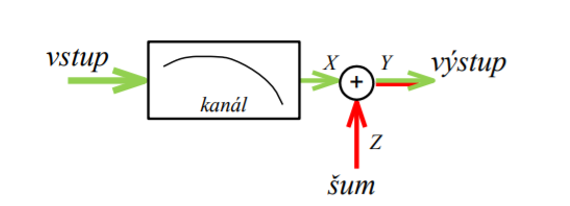
\includegraphics[]{images/AWGN.png}

\subsection{Uveďte a popište Shannonův vztah pro kapacitu kanálu. Za jakých podmínek byl odvozen: model, charakter signálu a šumu, Co je SNR a jak se většinou udává?}
$$C = B*log_2(1+SNR.)$$
Byl odvozen za podmínek platnosti Nyquistova kritéria a na modelu AWGN.
$$M \leqq 2B,$$ které říká, že potřebná šířka pásma je B je minimálně poloviční oproti modulační rychlosti M, anebo opačně maximální modulační rychlost M je rovna dvojnásobku šířky pásma.

\textbf{SNR} znamená tzv. odstup signál šum na straně přijámače, jednotkou je decibel[dB]

\subsection{Co je to modulační rychlost? Jakou má jednotku? Jaký je vztah mezi ní a šiřkou pásma}
viz. otázka 8.

Vztah mezi modulační rychlostí a šiřkou pásma
\begin{itemize}
    \item Pro spojitý kanál je popsán Nyquistovým kritériem
    \item $M \leqq 2B $, které říká, že potřebná šířka pásma B je minimálně poloviční oproti modulační rychlosti M anebo opačně maximální modulační rychlost M je rovna dvojnásobku šířky pásma.
\end{itemize}

\subsection{Co popisuje výkonová spektrální hustota, jakou má jednotku, v jakých jednotkách se zpravidla udává. Uveďte vztah pro výkon}
 Výkonová spektrální hustota popisuje rozložení výkonu napříč spektrem, Její základndí jednotkou je W/Hz. Většinou se ale uvádí v dBm/Hz

Vztah pro výkon
$$P = \int_{-\infty}^{\infty} PSD(f)\mathrm{d}f$$

\subsection{Pro jaké veličiny jsou běžně užívané jednotky dBm a dBm/Hz. Uveďte základní jednotky
těchto veličin a vztahy pro přepočet.}
\begin{itemize}
    \item dBm - pro výkon (vysílací nebo výkon šumu), základní jednotka je Watt [W] (poměr výkonu k 1 mW)
    \item Přepočet: $P_{dBm}=10\cdot log\left(\frac{P_W}{0,001}\right)$
    \item dBm/Hz - pro spektrální hustotu (signálu nebo šumu), základní jednotka je Watt/Hertz [W/Hz]
\end{itemize}

\subsection{Co je to problém příjemce}
Problém příjemce je zjištění, zda platí rovnost $S=S^*, $ kde S=${s_i}$ ze zdroje dat a $S^*$ je vstupní abeceda dekodéru.

\subsection{Obecný princip kódování a jeho vysvětlení.}
\begin{itemize}
    \item Používá se:
    \begin{itemize}
        \item kódování zdroje - pro vyjádření velkého počtu zpráv malým počtem stavů kanálu
        \item kódování kanálu - protichybové kódování, linkové kódy, modulace
    \end{itemize}
    \item Obecně jde o modifikaci dat jinými daty podle určitých pravidel
    \item U kódování zdroje jde o záměnu zpráv abecedy S na řetězce znaků abecedy X
    \item U kódování kanálu jde o přidávání do informačních dat délky $k$ zabezpečovací data délky $r$
\end{itemize}

\subsection{Co je to „Kódování zdroje“ a „Kódování kanálu“ }
\begin{itemize}
    \item \textbf{Kódování zdroje} -Představitelem tohoto typu kódování je kódování pro přizpůsobení zdroje na kanál z důvodu vyjádření velkého počtu zpráv určujících zdroj zpráv počtem stavů signálu přenositelného kanálem. Existují ale i jiné druhy kódování zdroje
    \item \textbf{ Kódování kanálu} - Je spojeno s vlastnostmi kanálu, který slouží k přenosu zprávy kanálem v podobě signálových prvků. K tomuto druhu kódování patří např. protichybové kódování, linkové kódy, modulace a další.
\end{itemize}

\subsection{Přehled druhů kódování v systémech pro přenos informace a jejich stručný popis}
\begin{itemize}
    \item  \textbf{Kódy pro přizpůsobení zdroje na kanál} - spojeny s realizací přenosového systému a musí být určeno
\begin{itemize}
    \item Definice vlastního kódu
    \item Definice způsobu přiřazení
\end{itemize}
\item \textbf{Kódy pro snižování nadbytečnosti} - některé kódy vytváří zprávy s vysokou redundancí = snižují přenosový výkon systému pro přenos informace. Řešení spočívá v přechodu na jinou, účinnější, abecedu zdroje.
\item Kódy pro zabezpečeení přenosu proti chybám
\item Kódy pro zrovnoměrnění spektra přenášenohé signálu - Scrambling
\item Kódy pro zabezpečení přenosu informace proti zcizení - šifrování
\end{itemize}

\clearpage
\section{Přenos dat}
\subsection{Vysvětlete pojmy značka, abeceda, kód, prvek značky a symbol}
\begin{itemize}
    \item \textbf{Značka} je skupina prvků ze souboru \textbf{X}, která je přiřazena v procesu kódování jednomu prvku ze souboru \textbf{S}.
    \item \textbf{Abecedu} definujeme jako množinu používaných značek.
    \item \textbf{Kód} je soustava dohodnutých pravidel, podle kterých mají být tvořeny, přenášeny a vyhodnocovány značky, odpovídající daným znakům.
    \item \textbf{Prvek značky} je elementární část značky, prvek ze souboru X
    \item \textbf{Symbol} je interpretace značky nebo její části v datovém signálu.
\end{itemize}

\subsection{Uveďte rozdíl mezi přenosovým kanálem a okruhem. Vysvětlete pojmy: komutovaný spoj, pevný spoj, simplexní, duplexní, poloduplexní spoj. Metody vytváření duplexního spojení}
\begin{itemize}
    \item \textbf{Přenosový kanál} - jde o soubor přenosových prostředků, který není přesně určen jen pro určitý druh přenosu, ale může být použit různými druhy přenosů využíván k  \textbf{jednosměrnému přenosu}.

    \item \textbf{Přenosový okruh} - Jde o soubor přenosových prostředků, který není přesně určen jen pro určitý druh přenosu, ale může být použit různými druhy přenosů využíván k \textbf{obousměrnému přenosu}.
    
    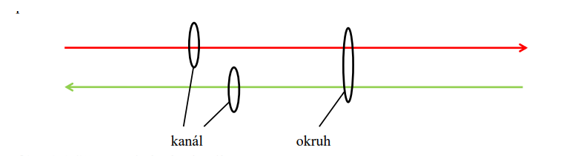
\includegraphics[]{images/okruh_kanal.png}
    
    \item \textbf{Komutovaný spoj} - jde o spoje, které se vytvoří před vlastním přenosem dat. př: spojení pomocí telefonních modemů nebo GPRS technologie.
    \item \textbf{Pevný spoj} - jde o trvalé spoje. Jejich nevýhoda spočívá ve snižování přenosové a spojovací kapacity systému vzhledem k ostatním uživatelům a proto je jejich realizace finančně náročná.
    \item \textbf{Simplexní spoje} - umožňují přenos signálu v jednom směru
    \item \textbf{Duplexní spoje} - umožňují současný přenos signálu v obou směrech
    \item \textbf{Poloduplexní spoje} - umožňují duplexní provoz, avšak pouze střídavě v jednom nebo druhém směru.
\end{itemize}
Metody realizace duplexního spojení
\begin{itemize}
    \item Kmitočtové
    \item Časové
    \item Obvodové
\end{itemize}

\subsection{Co jsou to provozní charakteristiky datových spojů. Popis nejčastěji užívaných}
\begin{itemize}
    \item \textbf{Přenosová rychlost} - potřebná rychlost závisí na potřebném objemu přenášených dat.
    Je odlišná na různých úrovních přenosu.
    Užitečná je někdy velmi výrazně nižší oproti udávané rychlosti fyzické.
    Dělí se dle dosažených maximálních rychlostí na malé, velké \dots.
    \item \textbf{Stálost přidělení spoje} - komutované a pevné.
    \item \textbf{Směr přenosu dat} - Podle směru rozlišujeme simplexní, duplexní a poloduplexní spoj.
    \item \textbf{Způsob přenosu značky}- podle časové realizace jednotlivých prvků rozlišujeme druhy přenosu
    \begin{itemize}
        \item \textbf{Paralelní způsob přenosu} - Všechny prvky značky se přenášejí ve stejném charakteristickém intervalu, po paralelních kanálech, kterých je stejný počet jako prvů ve značce.
        \item \textbf{Sériový způsob přenosu} - Prvky značky se přenášejí postupně za sebou po jednom kanálu.
        Tento způsob je náročný na čas potřebný k přenosu značky.
                
    \end{itemize}
    \item \textbf{ Časový režim přenosu}- V přijímači je nutno zajistit správné vyhodnocování značek, rozlišit jejich začátky a konec, tedy zajistit synchronizaci.
    Při sériovém přenosu se nejčastěji setkáme s těmito typy přenosu.
\end{itemize}

\subsection{Vysvětlete rozdíl mezi rychlostí přenosu $v_p$ a rychlostí přenosu informace $v_i$ v datových přenosech.
Jaký je rozdíl mezi jednotkami $[bit/s]$ a $[Sh/s]$.}
\textbf{Přenosová rychlost} je definovaná jako počet dvojkových signálových prvků (bitů) přenesených za 1 s. 
$v_p=M\cdot \log_2(F)$ $[bit/s]$, $M$ je modulační rychlost, F je počet stavů.

\textbf{Rychlost přenosu informace} - informační rychlost (průměrné množství informace za 1 s), $v_i=\frac{H_X}{t_p}$ 
$[Sh/s]$, $t_p$ je doba výstupu prvku z přizpůsobeného zdroje

$Sh$ se vztahuje k přenesené informaci, tedy k celé zprávě. Bit je prvek značky.

\subsection{Vysvětlete pojmy časového režimu přenosu: synchronní přenos a arytmický. Uveďte příklady}
\begin{itemize}
    \item  \textbf{Synchronní} - značky jsou vysílány kontinuálně a ke změně dochází po konstantním časovém intervalu.
    Není-li potřeba přenášet data přenáší se výplňové značky.
    \item \textbf{Arytmický} - vysílání může být zahájeno v jakémkoli okamžiku. 
    Počátek přenose se označuje specifická kombinace start a stop. Příkladem je rozhraní RS 232.
    
\end{itemize}

\subsection{Co je to systém přenosu dat. Jeho základní striktura a význam jednotlivých částí}
Jde o soubor podrobněji nespecifikovaných zařízení, které slouží k technické realizaci přenosu dat.
Tvoří jej hardware i software.

\includegraphics[]{images/přenos_dat.png}

\subsection{Specifikujte  4 základní typy rozhraní, které jsou zpravidla předmětem normalizace. Jaké znáte normalizační organizace}
\textbf{Typy rozhraní}
\begin{itemize}
    \item Mechanické vlastnosti -  rozměry a tvary dílů, typy konektorů
    \item Elektrické vlastnosti - úrovně napětí a proudu
    \item Funkční vlastnosti - význam jednotlivých signálů a jejich časové průběhy, včetně tolerancí
    \item Operační vlastnosti -  řídící, aplikační, testovací a diagnostické postupy
\end{itemize}
\textbf{Normalizační organizace}
\begin{itemize}
    \item ITU - International Telecommunication Union
     \item IETF - Internet Engineering Task Force
     \item IEEE - Institute of Electrical and Electronic Engineering
     \item ANSI - American National Standards Institute
     \item ETSI - European Telecommunications Standards Institute
\end{itemize}

\subsection{Popište vlastnosti a použití rozhraní RS232 a USB}
\textbf{RS232}
\begin{itemize}
    \item Standardní sériové rozhraní, dříve používáno pro připojení telefonních modemů.
    Dnes se využívá pro malé přenosové rychlosti, konfigurační rozhraní atd.
    V mnoha technologiích je pro standardní podporu softwarově emulováné, ač je přenos realizován jinými technologiemi.
\end{itemize}
\textbf{USB}
\begin{itemize}
    \item Jde o sériové rozhraní, které se některých aplikacích nahrazuje dřive používané rozhraní.
    USB tvoří sběrnici s jedním zařízením typu Master a ostatní typu Slave.
    Můžeme se setkat s několika standardy:
\begin{itemize}
    \item Low speed
    \item Full speed
    \item High speed
    \item Super speed
\end{itemize}
\end{itemize}
\subsection{Ve kterých technologiích se můžete setkat s konektorem RJ45}
\begin{itemize}
    \item Ethernet přes UTP
    \item Rozhraní E1 - používané v telekomunikacích pro přenos 30 hovorových kanálů.
    \item Sériové rozhraní RS232 - viz. výše.
\end{itemize}
\subsection{Uveďte příklady sériových sběrnic pro mikrokontrolery}
\begin{itemize}
    \item I$^2$ C - Inter-integrated circiut - jde o sběrnici používající dvojice signálových vodičů v zapojení s otevřeným kolektorem SCLK a SDA
    \item SPI- Serial Peripheral Interface Bus - jde sběrnice využívající trojice signálů SCLK, MOSI a MISO
\end{itemize}

\section{ Vysvětlete základní princip snižování nadbytečnosti}
Při realizaci přizpůsobení zdroje na kanál pomocí rovnoměrného kódování dochází k vyoké nadbytečnosti -> menší účinnost.
Řešením tohoto problému je využití nerovnoměrného kódování, které znakům s častějším výskytem přiřazuje značku s menším počtem bitů -> zkrácení doby přenosu oproti rovnoměrnému kódování -> zkrácení střední délky značky a zvýšení průměrné entropie na jeden bit zprávy.

\section{Co je to prefixový kód? Popište způsob dekódování.}
\begin{itemize}
    \item Prefixový kód je \textbf{nerovnoměrný kód}, pro nější platí, že žádná značka není prefixem jiné značky.
    \item Kódování se nazývá prefixovo, pokud je \textit{prosté}, tj. je realizováno prostým přiřazením a žádná značky není prefixem jiné značky.
    \item \textbf{Pokud je kód prefixový, je jednoznačně dekódovatelný}

\end{itemize}
\textbf{Dekódování}
\begin{itemize}
    \item Po přijmutí značky v ní najdeme nejmenší počet signálových prvků (zleva), které tvoří některou z užívaných značek.
    Tím považujeme první zprávu za dekódovanou a tyto prvky "umažeme".
    Poté opět hledáme nejmenší počet signálových prvků (opět zleva), které tvoří nekterou z užívaných značek a získáváme druhou zprávu \dots
\end{itemize}

\section{Co specifikuje Kraft-McMilanovo číslo, Kraftova nerovnost a McMilanova věta}
Mějme kód definovám předpisem S->X, poté \textbf{KraftMilanovo číslo} specifikuje
\begin{itemize}
    \item m$_i$ - počet symbolů v S, které jsou kódovány řetěžci dělky \emph{i} z množiny X.
    \item M - maximální délka kódovaného slova užívající F prvkového tělesa
    $$K = \sum_{i=1}^M \frac{m_i}{F^i}= \frac{m_1}{f} + \frac{m_2}{F^2} \dots \frac{m_M}{F^M}$$
\end{itemize}
\textbf{McMilanova věta}
\begin{itemize}
    \item Pro jednoznačně dekódovatelný kód platí Kraftova nerovnost $K \leqq 1$
    \item Věta však neplatí obráceně.
    I pří K < 1 nemusí být kód jednoznačně dekódovatelný.
    Z McMilanovy věty vychází
    \begin{itemize}
        \item K < 1 - kód nemá nadbytečnost a může být jednoznačně identifikován
        \item K = 1 - jedná s o tzv. kompletní kód a může být jednoznačně identifikován.
        \item K > 1 - kód není jednoznačně dekódovatelný
    \end{itemize}
\end{itemize}
\section{Uvěďte příklady algoritmů pro bezztrátovou kompresi}
\begin{enumerate}
    \item Aritmetické kódování (délka značek podle jejich pravděpodobností)
    \item Kódování s dynamickým slovníkem (LZW algoritmus)
\end{enumerate}

\section{Co je optimální kód, pomocí které veličiny můžeme tyto kódy porovnávat}
Nalezení optimálního kódu vede  na optimalizační problém, což je hledání minimální střední délky značky změnou délek jednotlivých $n_1, n_2, n_3 \dots n_n$, pro známí soubor pravděpodobností $p_1, p_2, \dots p_n$ pří splnění Kraftovy nerovnosti
$$\Bar{n}_{opt} = min \{\Bar{n}\},$$ kde
$$\Bar{n}=\sum_{i=1}^q p_i*n_i$$ a 
$$K\leqq1$$
Tedy hledáme takové délky $n_1=? \dots n_n=?$ pro zadané $p_1,p_2\dots p_n$ pro které je střední délka značky minimální, je splněna Kraftova nerovnost a kód je jednoznačně dekódovatelný, tj. prefixový.

Kódy lze porovnávat podle $\Bar{n}_{opt}$ (?)

\section{vysvětlete princip Huffmanova kódu}
Kód je založen na Huffmanově pravidle, které umožňuje navržení optimálního kódu.

\begin{enumerate}
    \item V množině symoblů primárního zdroje vyhledáme dva symboly s nejmenší pravděpodobností a sloučíme je.
    \item U původních symbolů si poznačíme 0 a 1
    \item Kroky 1) a 2) opakujeme dokud nevytvoříme zdroj s pouze jedním prvkem
    \item Kódová slova vytváříme zpětným procházením vytvořeného stromu a zapisováním si 0 a 1.
\end{enumerate}

\section{Vysvětlete princip a důvod použítí kódování bloků dat}
Může nastat situace, že množina prvů zdrojové abecedy S je menší než množna prvků pomocného zdroje X->q->F, nebo je počet prvků zdrojové abecedy moc malý pro provedení efektivní datové komprese.
Příkladem může být černobílý obrázek, který je složený ze 2 prvků zdrojové abecedy černého a bílého bodu.
V takovém případě můžeme využít sloučení více prvků primární abecedy a vytvořit tak novou sadu s vyšším pročem prvků.

\section{Vysvětlete princip Aritmetického kódování a porovnejte s Huffmanovým kódem}
\begin{itemize}
    \item \textbf{Aritmetické kódování} realizuje návrh značky pro každý symbol primární abecedy individuálně, což umožňuje efektivně modifikovat l´d v případě změny v jejím výskytu.
    \item V tomto kódování se využívá vyjádření reálného čísla v rozsahu (0,1) v binrním vyjádření ve tvaru
    $$0.x_1x_2x_3\dots x_n=\frac{x_1}{2}+\frac{x_2}{2^2}+\dots+\frac{x_n}{2_n}$$
\end{itemize}
Narozdíl od huffmanova kódu aritmetické kódování navrhuje značku pro každý symbol primární abecedy individuálně -> v mnoha případech je nebo může být efektivnější než Huffmanovo kódování.
\section{Vysvětlete rozdíl mezi kódováním s dynamickým a statistickým slovníkem. Uveďte příklady kompresních algoritmů a zařaďte je do těchto skupin}
\begin{itemize}
    \item  \textbf{Statistický slovník} - Kódovací předpis musí být znám před vlastním přenosem - aritmetické kódování
    \item \textbf{Dynamický slovník} - Předpis je vytvářen dynamicky během přenosu ( algoritmus LZW
\end{itemize}

\section{Vysvětlete princip LZW kódování}
\begin{enumerate}
    \item První symbol $z_1$ tvoří prvek $s_p$ zdrojové abecedy a tedy \emph{p}-tý prvek $d_p$ počátečního slovníku D$_0$.
    První prvek vytvářeného kódu bude:$c_1 = p$.
    Řetězec $z_1, z_2$ kódovací slovník zatím neobsahuje.
    Definujeme tedy další řetězec kódovacího slovníku $d_{q+1} = z_1, z_2$ a nový slovník $D_1=(D_0,d_{q+1}) $
    \item Ve všech následujících krocích budeme hledat nejdelší řetězec $w = z_i+1\dots z_j$ $(j\geqq i+1)$ v aktuálním slovníku D.
    Tvoří-li její \emph{r}-tý prvek $d_r$, bude dalším prvkem kódu $c_i=r$. 
    Opět definujeme další prvek slovníku w $z_{j+1}$ a vytvoříme tak nový slovník $D_{i+1} = (D_i, w\mathrm{ }z_{j+1}$.
    \item Algoritmus nevyžaduje žádný slovník, definuje si sám seznam frází, které skládá. Vznikají hledáním a prodlužováním jižpoužitých frází.
\end{enumerate}

\clearpage
\section{Protichybové kódování}
\subsection{Uveďte, jaké rušivé vlivy mohou působit na přenos}
\begin{itemize}
    \item \textbf{Šum} - náhodné změny fyzikální veličiny, které nepříznivě ovlivňují přenášený signál.
    \item \textbf{Rušení} - nepříznivé ovlivnění přenášeného signálu jiným elektrickým systémem.
    \item \textbf{Hluk} - Jde o všechny dynamické vlivy kanálu, které působí nepříznivě na přednášený signál
    \item \textbf{Šum} a rušení jsou podmnožinou obecného termínu hluk
    \item Významné rušivé jevy
    \begin{itemize}
        \item Jde o takové ručivé jevy, které mají náhodný charakter a velkou výkonovou  úroveň - impulsivní hluk, krátkodobý pokles úrovně signálu a krátkodobá změna fáze
        \item \textbf{Impulsní hluk} - Nejnebezpečnější.
        Má charakter krátkých vysokofrekvenčních kmitů o značné amplitudě, které se střídají s delšími bezhlukovými intervaly. Nebezpečí spočívá v relativně velké výkonové úrovny ve vztahu k přenášenému signálu a náhodnosti jeho charakteru.
    \end{itemize}
\end{itemize}

\subsection{Uveďte, proč je impulsní hluk považován za nejnebezpečnější}
viz. přechozí otázka

\subsection{Uveďte a popiště model vzniku chyb}
Zpráva je přenášena nejčastěji jako posloupnost dvou signálových prvků, kterým jsou přiřazeny hodnoty 0,1.
Chyby se projevují v posloupnosti dvoustavových signálových prvků jako inverze hodinty signálového prvku, tj. 0->1, 1->0.

Rušení se projeví inverzí hodnot určitých prvků, což můžeme modelovat pomocí sčítačky modulo 2

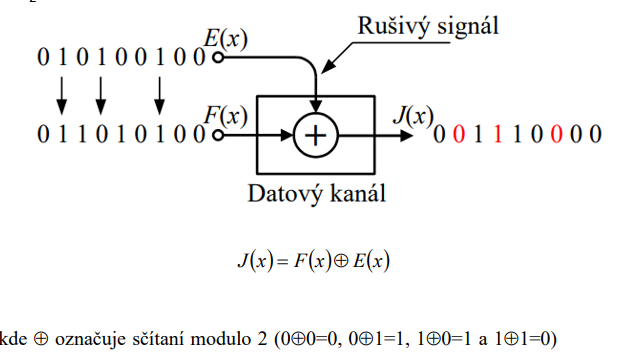
\includegraphics[]{images/ručení.png}
\begin{itemize}
    \item E(x) je chybová posloupnost - její strukturu zjišťujeme jako rozdíl F(x) a J(x).
    \item F(x) - posloupnost nul a jedniček přivedena na vstup datového kanálu.
    \item J(x) - posloupnost jedniček a nul na výstupu
    \item Je li přenost bezchybný, pak F(x) = J(x) a E(x) je posloupnost 0.
    \item K zápisu F(x),E(x) a J(x) se využívá mnohočlenů
\end{itemize}
\subsection{Vysvětlete pojmy: nezávislé chyby, shluky chyb, bitová chybovost, bloková chybovost}
\textbf{Nezávislé chyby} - Jejich rozložení je v přijaté zprávě relativně rovnoměrné.
Má tedy váznam hledat různé statistické odchylky
\begin{itemize}
    \item \textbf{Jednoduchá chyba} - Vyjadřuje skutečnost, že v signálu o \emph{n} prvků je pouze jeden prvek chybný
    \item \textbf{Vícenásobná chyba} - Vyjadřuje skutečnost, že v posloupnosti \emph{n} signálových prvlů se vyskytuje několik nezávislých chyb
\end{itemize}

Shluky chyb jsou takové úseky chybně přenesených prvkům ve kterých relativní četnost chybně přenesených prvků výrazně převyšuje četnost chybných prvků ve zbytku zprávy.
Počet chybných prvků ve shluku vyjadřujeme pomocí hustoty chyb shluku v \%

\subsection{Co udává kódový poměr a kódový zisk. Co je Shannonův limit}
Kódový poměr - Poměr informačních bitů ku všem přeneseným (včetně zabezpečovacích)

\textbf{Kódový zisk} - protichybové kódování umožňuje snížit odstup SNR(odstup signál-šum) při udržení stejné chybovosti.
Poměr potřebného SNR$_{NEKOD}$ ku SNR$_{KOD}$ s kódováním se označuje jako kódový zisk. 
Jeho jednotkou je [dB].

\textbf{Shannonův limit} říka, že pro daný kódový poměr R musí být dosažena určita minimální hodnota SNR.
Tato minimální hodnota se nazývy Shannonův limit, je uvedena v [dB].

\subsection{Uveďte základní dva typy protichybových kódových systémů, jejich výhody a nevýhody}
\begin{itemize}
    \item \textbf{Zabezpeční pomocí opravných protichybových kódů:} Metoda vyžaduje pouze jednosměrný přenos dat.
    Vložená nadbytečnost ve vysílači umožňuje chyby v přijímači opravit
    \item \textbf{Zabezpečení pomocí detekčních protichybových kódů s opakováním chybného přenosu - Automatic Repeat Request: }každá přenesená sekvence dat je potrvzována přijímačem.
    Při chybě je chybná sekvence zopakována.
    Existuje několik metod ARQ - Stop-and-Wait, go-back, selective
\end{itemize}
\subsection{Vysvětlete rozdíl mezi zabezpečením blokovým a stromovým kódem}
\begin{itemize}
    \item \textbf{Blokové kódy:} Zabezpečovací proces je realizován pouze v rámci jediného bloku dat, který vznikl rozdělením datového toku do úseků o definovaném počtu k-signálových prvků.
    \item \textbf{Stromové kódy: }Zabezpečovací proces je realizován nejen na základě jediného bloku dat, ale využívá se k němu navíc m-1 předchozích k-prvkových bloků dat.
    Vzniklá závislost zabezpečovací sekvence je dalším zapezpečovacím prvkem.
\end{itemize}

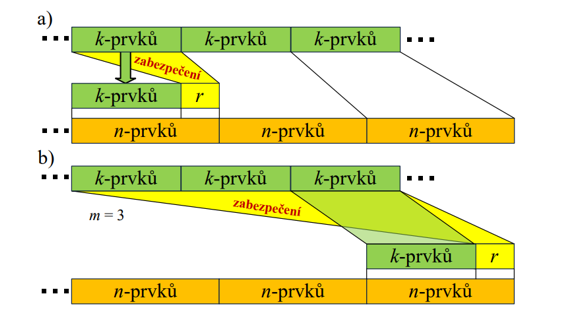
\includegraphics[]{images/zabezpečování.png}

\subsection{Co udává hammingova vzdálenost a váha? Vyvětlete využití}

\begin{itemize}
    \item \textbf{Hammingova vzdálenost (d):} Udává počet míst, ve kterých se dvě kombinace prvků ve sledovaném úseku zprávy mezi sebou liší.
    

    
    \item \textbf{Hammingova váha (w):} Udává počet nenulových prvků v kódovém slove.
    Minimální Hammingova váha je nejmenší váha mezi všemi kódovými slovy kromě slova s nulovými prvky.
    
    \item Využívá se v protichybovém kódování, kde uměleje snižujeme $d_{min}$ tak, že k signálovým prvkům nezabezpečené zprávy přidáváme zabezpečovací prvky podle pravidel definujicích použitý protichybový kód.
    Jiná možnost dosažení d$_{min}$ spočívá ve výběru takových posloupností signálových prvků ze všech možných posloupností signálových prvků délky n rozdělí na užívané posloupnosti, které tvoří protichybový kód a neužívané posloupnosti.  Při tomto způsobu tvorby kódu můžeme rozlišit původní nezabezpečené prvky a zebezpečovací prvky.
\end{itemize}
\subsection{Vysvětlete princip zabezpečení zpráv proti chybám a a jeho vysvětlení}
Uměle přidáváme další bity ke značkám, které zvětšují Hammingovu vzdálenost těchto značek a díky tomu při chybě jsme schopni určit, kde chyba nastala.

\subsection{Co určuje Plotkinova hranice + vztahy a další kritéria}
Používá se k určení minimální potřebné délky kódového slova k dosažení požadované korekční či detekční schopnosti kódu. Zabezp. r = n - k
$$n \geq 2* d_{min} -1$$
$$r \geq 2* d_{min} -  log_{2}  d_{min} -2$$
Pomocí \textbf{SF pravidla}, lze vypočítat délky jednotlivých značek: $n_{i} = -log_{2}p_{i}$

Pro hledání optimálního kódu, lze využít \textbf{Kraft-McMillanovo číslo K} a \textbf{Kraftovu nerovnost.}

\clearpage
\section{Blokové kódy}
\subsection{Stručně charakterizujte druhy blokových kódů.} \label{druhy}
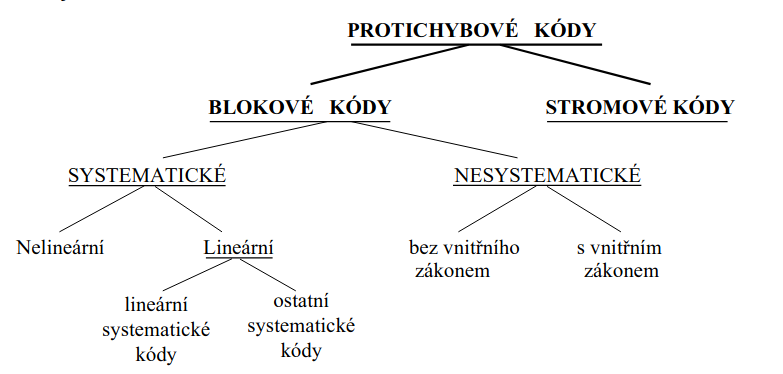
\includegraphics[width=16cm]{images/6_druhy.png}
\begin{itemize}
    \item systematické - rozložení informačních a zabezpečovacích bitů je stejné
    \begin{itemize}
        \item nelineární - nejsou lineární, vznikají např. kódovací tabulkou
        \item lineární - libovolnou kódovou kombinaci lze odvodit jako lineární kombinaci z ostatních kódových kombinací
        \begin{itemize}
            \item lineární systematické kódy - napřed se pošlou informační a na konci bloku jsou bity zabezpečovací
            \item ostatní lineární kódy - zabezpečovací bity jsou mezi informačními, na definovaných pozicích
        \end{itemize}
    \end{itemize}
    \item nesystematické - nerozlišují informační a zabezpečovací bity, zabezpečení spočívá v Hammingově vzdálenosti
    \begin{itemize}
        \item bez vnitřního zákona - správnost se ověřuje jen srovnáním s používanými bloky
        \item s vnitřním zákonem - mají jednoduché pravidlo určení správnosti přenosu (např. \uv{počet jedniček v bloku je 7})
    \end{itemize}
\end{itemize}

\subsection{Vysvětlete pojem lineární systematický blokový kód. Co znamená pojem lineární, co systematický a co blokový v problematice protichybových kódů?}
\begin{itemize}
    \item \textbf{Blokové kódy} - zabezpečovací proces je realizován pouze v rámci jediného bloku dat, který vznikl rozdělením datového toku
    \item \textbf{Systematické kódy} - můžeme zcela jednoznačně rozlišit v posloupnosti přenášených prvků informační prvky $k$ a zabezpečovací prvky $r$
    \item \textbf{Lineární kódy} - libovolnou kódovou kombinaci lze odvodit jako lineární kombinaci z ostatních kódových kombinací
\end{itemize}

\subsection{Podrobnější třídění blokových kódů a stručná charakteristika druhů blokových kódů.}
(viz. \ref{druhy})

\subsection{Co musí platit pro řádky vytvářecí matice lineárního blokového kódu. Jak vektory tvořící tyto řádky označujeme?}
\begin{itemize}
    \item Vytvářecí matice G má k řádků a n sloupců
    \item Řádky tvoří kódové kombinace, které jsou vzájemně lineárně nezávislé, tj. žádnou lineární operací mezi libovolnými řádky matice G nevznikne jiný řádek této matice
    \item Žádný z řádků matice nesmí obsahovat pouze nulové prvky
    \item Porovnáním řádků matice lze určit minimální Hammingovu vzdálenost $d_{min}$, která odpovídá minimální Hammingově vzdálenosti kódu $d_{min}$
    \item \textbf{Řádky} = generující vektory (báze vektorového prostoru)
    \item $G*H^{T}=0$
\end{itemize}

\subsection{Jaký je obecně vztah mezi vytvářecí a kontrolní maticí? Co tento vztah z hlediska
vektorových prostorů znamená?}
\begin{itemize}
    \item Vytvářecí matice $G=[I_{k\times k} C_{k\times r}]$, kde $I$ je jednotková matice, $C$ je zabezpečovací matice.
    \item Kontrolní matice $H=[C^T_{r\times k} I_{r\times r}]$ nebo ve tvaru $H^T=\left[ \begin{array}{cc}
        C_{k\times r} \\
        I_{r\times r}
    \end{array}\right]$
    \item $H$ generuje ortogonální vektorový prostor vůči $G$, platí $G\cdot H^T=0$
\end{itemize}

\subsection{Zapište maticově proces kódování a dekódování.}
\begin{itemize}
    \item kódování: $f=p\cdot G$, kde f je vysílaný blok
    \item dekódování: $j\cdot H^T=s$, kde j je přijatý blok a s je syndrom
\end{itemize}

\subsection{Vysvětlete princip funkce zapojení kodéru lineárního blokového kódu.}
$G=\left[\begin{array}{ccccccc}
    1 & 0 & 0 & 0 & 1 & 0 & 1 \\
    0 & 1 & 0 & 0 & 1 & 1 & 1 \\
    0 & 0 & 1 & 0 & 1 & 1 & 0 \\
    0 & 0 & 0 & 1 & 0 & 1 & 1
\end{array} \right]$, $r_1=p_1 \oplus p_2 \oplus p_3$ (první zabezpečovací bit je součet prvních 3 vstupů,
protože jedničky ve sloupci zabezpečovacího bitu $r_1$ jsou jedničky na 1., 2. a 3. řádku. Obdobně pak:
$r_2=p_2\oplus p_3 \oplus p_4$ a $r_3=p_1 \oplus p_2 \oplus p_4$\\
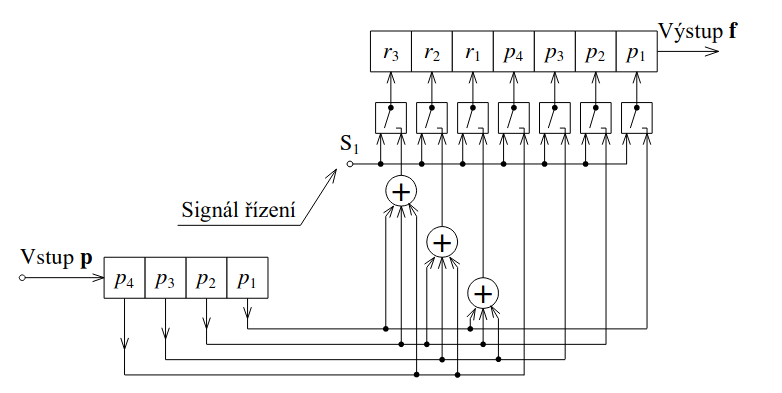
\includegraphics[width=16cm]{images/6_koder.png}

\subsection{Co je to syndrom. Vysvětlete vztah mezi syndromem, kontrolní maticí a chybovým
vektorem. Jak lze vytvořit tabulku syndromů?}
\begin{itemize}
    \item Syndrom je výsledek násobení přijatého vektoru s transponovanou kontrolní maticí. 
    Jedná se o kontrolu správnosti.
    \item Kontrolní matice slouží ke kontrole přijaté zprávy, generuje syndrom.
    \item Chybový vektor je binární vektor, označuje na kterých bitech došlo při přenosu k chybám. K jeho 
    nalezení slouží syndrom. Chybový vektor obsahuje jedničky na těch bitech, jejich pořadí odpovídá řádku transponované
    kontrolní matice, který je stejný jako syndrom. (např. třetí řádek kódu (7, 4) je [0 1 1], syndrom je stejný,
    chybový vektor je [0 0 1 0 0 0 0]
\end{itemize}

\subsection{Vysvětlete princip funkce zapojení dekodéru lineárního blokového kódu.}
Dekodér se skládá ze vstupní paměti, generátoru syndromu, generátoru chybového vektoru a korekce. Proběhne
maticové násobení, z něhož je nalezen syndrom. Ze syndromu nalezneme chybový vektor a ten přičteme 
k přijaté posloupnosti.

\subsection{Uveďte a vysvětlete jakým způsobem, jakou maticí jsou definovány základní Hammingovy kódy?}
\begin{itemize}
    \item Délka kódové kombinace: $n=2^m-1$
    \item r: $m$
    \item k: $2^m-1-m$
    \item $m \geq 3$
    \item Kontrolní matice je počítána binárním zápisem čísel do sloupců. Např. kód (7, 4):\\
    $H=\left[\begin{array}{ccccccc}
        0 & 0 & 0 & 1 & 1 & 1 & 1 \\
        0 & 1 & 1 & 0 & 0 & 1 & 1 \\
        1 & 0 & 1 & 0 & 1 & 0 & 1
    \end{array}
    \right]$
    \item Transponovaná matice $H^T$ vznikne jednoduchým transponováním.
    \item Zabezpečovací bity: $r_1 = 3 \oplus 5 \oplus7$, $r_2 = 3 \oplus 6 \oplus 7$,
    $r_3 = 5 \oplus 6 \oplus 7$ (od druhé jedničky na každém řádku kontrolní matice, číslování řádků odspodu)
\end{itemize}

\clearpage
\section{Blokové cyklické kódy}
\subsection{Čím se liší cyklický a blokový kód?}
Cyklický kód je určen namísto vytvářecí matice G vytvářecím mnohočlenem G(x).
Vytvářecí matice G některých lineárních kódů jdou převést součty mezi řádky do takového tvaru, že každý řádek obsahuje stejné prvky, pouze o jedno místo posunuté v jednom směru.

\subsection{Vysvětlete vazbu mezi vytvářecí maticí a vytvářecím mnohočlenem.}

\subsection{Matematický zapište proces kódování a dekódování cyklickým kódem.}

\subsection{Uveďte některé cyklicky definované kódy.}
CRC kódy, cyklické kódy odvozené z Hammingova kódu, Fireův kód 

\subsection{Zapojení dekodéru cyklického detekčního kódu.}

\subsection{Vysvětlete princip Meggitova dekodéru. Pro které kódy jej lze využít?}

\subsection{Vysvětlete pojem Galoisovo těleso a uveďte, které kódy jej využívají?}
Pomocí prvků tohoto tělesa se uskutečňují operace spojené se zabezpečováním posloupnosti nezabezpečených signálových prvků. Galoisova tělesa GF (p$^r$). Zde $p$ je základ číselné soustavy (2) a $r$ odpovídá počtu zabezpečovacích prvků v mnohočlenu zabezpečené zprávy. Je tvořeno konečným počtem prvků n = p$^r$  a vzniklo rozšířením tzv. konečného tělesa Zp.

BCH kódy, Reed-Solomonovy (RS) kódy

\clearpage
\section{Stromové kódy}
\subsection{Popište základní vlastnosti stromových kódů a odlišnost oproti blokovým.}
Stromové kódy mají jiný způsob zabezpečení datového toku v porovnání s kódy blokovými. 
Dalším prvkem zabezpečení zde, krom vkládání nadbytečných prvků, je jejich závislost na předchozích 
informačních prvcích nezabezpečeného datového toku. \\
Parametry:
\begin{itemize}
    \item $k_0$ počet bitů ve vstupním bitovém úseku
    \item $n_0$ počet bitů ve výstupním bitovém úseku
    \item informační rychlost $R=\frac{k_0}{n_0}$
    \item délka kódového ohraničení $\nu=m\cdot k_0$ (viz. \ref{nu})
    \item Nezabezpečený blok stromového kódu $k=(m+1)\cdot k_0$
    \item Zabezpečený blok stromového kódu $n=(m+1)\cdot n_0$
\end{itemize}


\subsection{Vysvětlete zadávání konvolučních kódů vytvářecími mnohočleny.}
Používáme operátor zpoždění $D$, jednotlivé mnohočleny mají v horním indexu vstupní tok, v dolním výstupní tok.
Znázorňují vazbu mezi vstupy a výstupy pomocí operátoru zpoždění. Příklady:
\begin{itemize}
    \item $G^{(i)}_{(j)}(D)$ - obecný zápis
    \item $G^{(1)}_{(1)}(D)=1+D$, $G^{(1)}_{(2)}(D)=1+D^2$ apod.
\end{itemize} 

\subsection{Vysvětlete zadávání konvolučních kódů vytvářecími maticemi.}
Vstupní toky jsou řádky matice $P$, výstupní pak $F$, vytvářecí matice je $G$. Platí $F=P\cdot G$. $G$ je
polonekonečná, protože je ohraničená délkou zprávy, která teoreticky může být i nekonečná. $G\infty$ 
se skládá z dílčích vytvářecích matic $G_t$, které mají $k$ řádků a $n$ sloupců. $G$ Umožňuje přepočítat sloupec 
vstupní matice $P$ pro časový okamžik $t$ na sloupec výstupní matice $F$ pro stejný časový okamžik. Ze vztahu (8.11) je zřejmé, že k popisu kódu pomocí $G\infty$ nám stačí znát sestavu matic $G_t$ pro $t = 1, 2, \dots, m$. \\
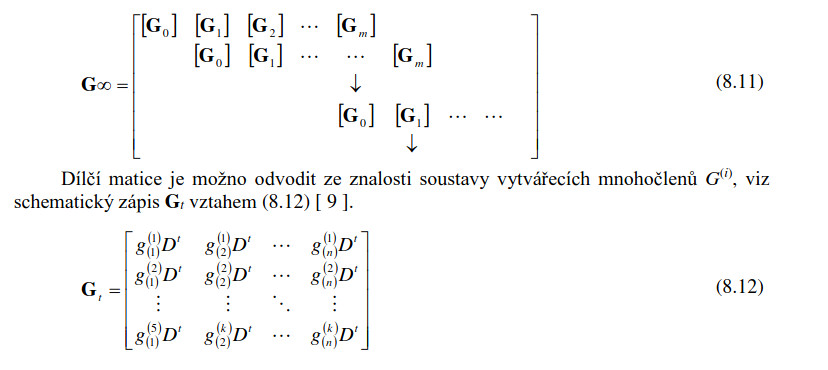
\includegraphics[width=16cm]{images/8_matice.png} \\
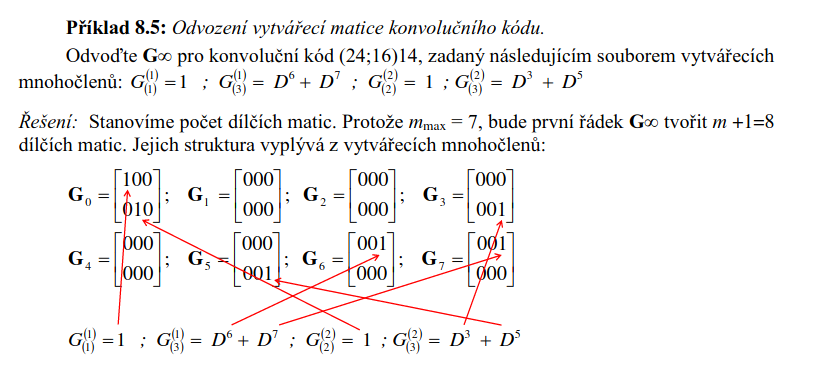
\includegraphics[width=16cm]{images/8_odvozeni.png}

\subsection{Vysvětlete princip a popište stromový graf.}
Graf znázorňuje vstupní bit, hodnoty pamětí a výstupní posloupnosti.\\
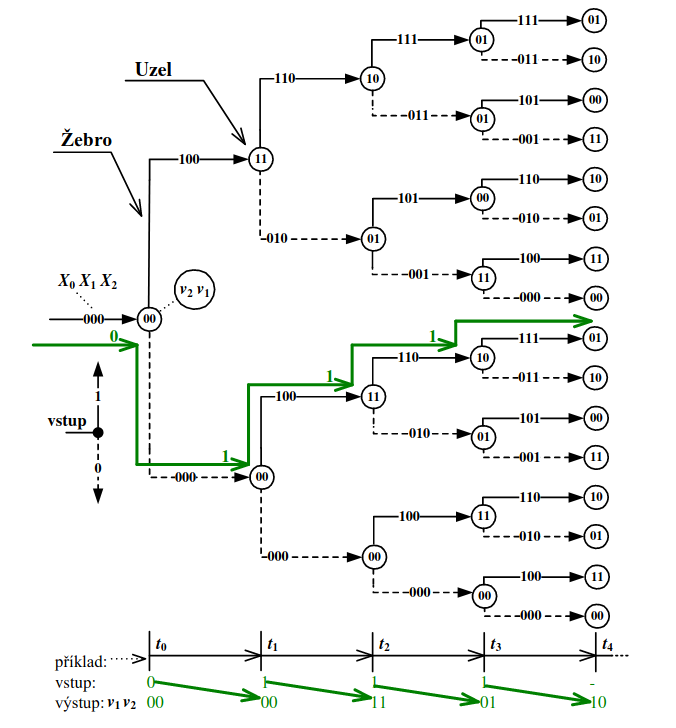
\includegraphics[width=16cm]{images/8_strom.png}

\subsection{Vysvětlete princip a popište mřížový graf.}
Podobný jako stromový, nerozvíjí se do nekonečna, ale opakuje se, když jsou v paměti všechny možnosti. \\
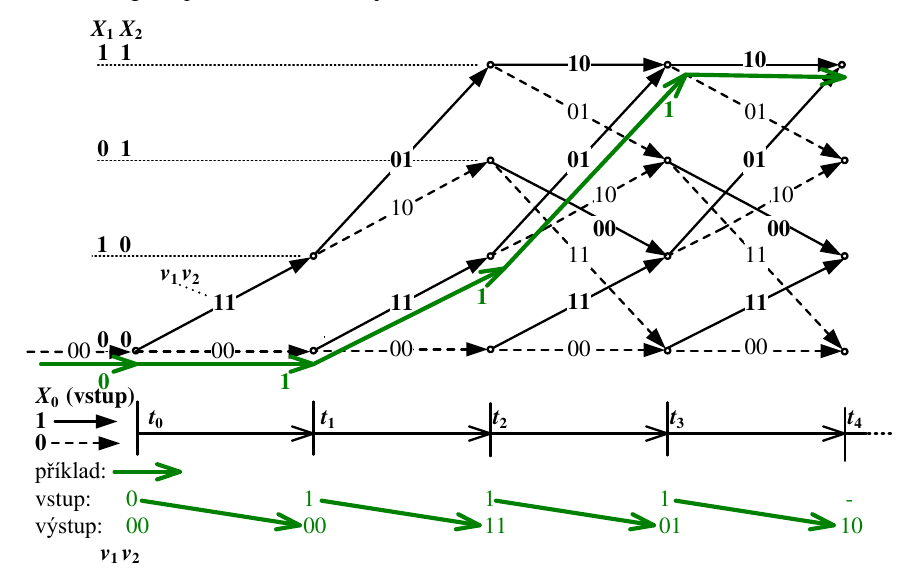
\includegraphics[width=16cm]{images/8_mriz.png}

\subsection{Vysvětlete princip a popište stavový diagram.}
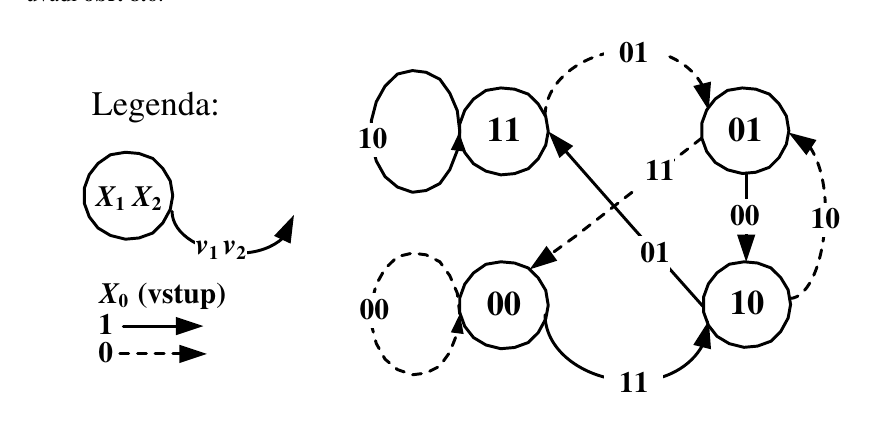
\includegraphics[width=16cm]{images/8_stav.png}

\subsection{Vysvětlete princip prahového dekódování konvolučního kódu.}
\begin{itemize}
    \item = syndromové dekódování
    \item Kontrolní matice $H\infty$ slouží k nalezení syndromu $s\infty$
    \item Kontrolní proces: $H\infty\cdot j\infty^T=s\infty^T$
    \item proces:
    \begin{itemize}
        \item Převedení sériového vstupu na paralelní
        \item Rozdělení na informační a zabezpečovací bity každého paralelně uspořádaného úseku
        \item Z informačních bitů se odvodí nové zabezpečovací bity a porovnají se s přijatými v generátoru syndromu
        \item Pokud došlo při přenosu k chybě, syndrom obsahuje informace o její poloze.
    \end{itemize}
\end{itemize}
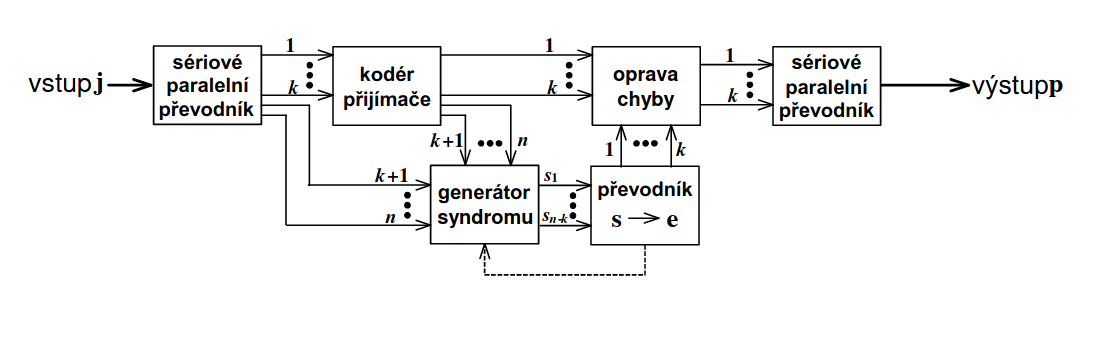
\includegraphics[width=16cm]{images/8_syndromove.png}

\subsection{Vysvětlete princip postupného pravděpodobnostního dekódování konvolučního kódu.}
\begin{itemize}
    \item Porovnává přijatou zprávu se seznamem užívaných zpráv a hledá nejmenší odchylku.
    \item Vhodná vizualizace procesu je dekódování pomocí mřížového grafu.
    \item Vzdálenost nejpravděpodobnější možnosti a přijatou zprávou je tzv. \textit{cena cesty}.
    \item U binárních kódů odpovídá cena cesty Hammingově vzdálenosti.
    \item typy:
    \begin{itemize}
        \item Postupné dekódování - o správnosti se rozhoduje prvek po prvku
        \item Dekódování po úsecích - o správnosti se rozhoduje po úsecích, Viterbiho algoritmus
    \end{itemize}
\end{itemize}

\subsection{Vysvětlete princip Viterbiho dekódovacího algoritmu.}
\begin{itemize}
    \item Po úsecích
    \item Úseky jsou porovnávány s používanými úseky v mřížovém grafu.
    \item Vybere se cesta s nejmenší cenou, z ní se odvodí informační prvky.
    \item Ochranná dekódovací hloubka $\mu$ by měla být 4 až 5 násobek kódového ohraničení $\nu$
    \item To, co jsme dělali v počítačových cvičeních
\end{itemize}

\subsection{Co je to délka kódového ohraničení $\nu$? Jaká je souvislost této délky a ochranné
dekódovací hloubky, při využití Viterbiho diagramu?} \label{nu}
\begin{itemize}
    \item Vyjadřuje, jak dlouho se bit podílí na zabezpečovacím procesu, vyjádřeno v bitech.
    \item Také určuje počet paměťových buněk paměti zabezpečovacího zařízení.
    \item Nezabezpečený blok stromového kódu $k$ je větší o 1 blok $k_0$, protože se na tvorbě podílí jeden 
    neuložený blok navíc.
    \item Z důvodu spolehlivosti by měla být u Viterbiho algoritmu ochranná dekódovací hloubka $\mu$
    4 až 5 násobek kódového ohraničení $\nu$.
\end{itemize}
\clearpage
\section{Turbo kódy}
\subsection{Uveďte a popište metody modifikace kódů.}
Nejběžnější metody modifikace kódů jsou: Zkracování kódů, rozšiřování kódů, děrování kódu, zvětšení kódu, zmenšení kódu, kombinování kódů a zřetězené kódy.
\begin{itemize}
    \item \textbf{Zkracování} - Princip zkrácení kódu spočívá ve zmenšení počtu využívaných kódových kombinací. Prvních $s$ prvků původního kódu je nulových a nepřenáší se - odstranění informačních prvků.
    \item \textbf{Rozšiřování} - Obecně rozšíření kódu spočívá v přidání $e$ zabezpečovacích prvků. Nejčastějším způsobem rozšiřování kódu je přidání paritního prvku
    \item \textbf{Děrování} - Děrování spočívá v odstraňování zabezpečovacích prvků, v Turbo kódech.
    \item \textbf{Zvětšení a zmenšení kódu} -  Vedou k nelineárním kódům. Zmenšování (zvětšování) kódu spočívá v odstranění (přidání) některých kódových slov z kódu.
    \item \textbf{Kombinování} - např. sčítat kódové kombinace různých kódů
    \item \textbf{Zřetězení} - také kombinování; výsledný zabezpečený datový tok z prvního kodéru je následně ještě jednou zabezpečen dalším kódem.
\end{itemize}

\subsection{Podrobněji vysvětlete metodu zkracování kódu.}
Je-li původní kód (n, k, d), vhodnou volbou celého čísla s v rozsahu $0 \leq s < k$ jej
zkrátíme na kód (n - s, k - s, ds), kde Hammingova vzdálenost zkráceného kódu ds je $ds \geq d$.
Vytvářecí matici zkráceného kódu Gs tvoří s+1 až k-tý řádek a s+1 až n-tý sloupec vytvářecí
matice G zkracovaného systematického lineárního blokového kódu. \\
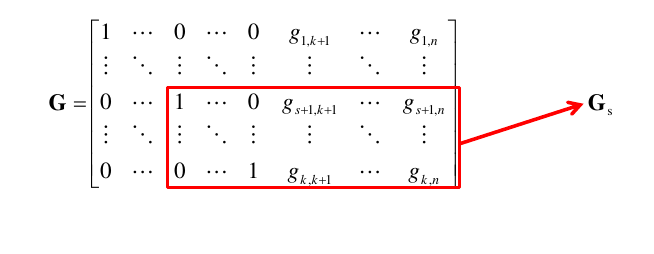
\includegraphics[width=16cm]{images/9_zkrac_obecne.png}\\
Např.: kód (7,4):\\
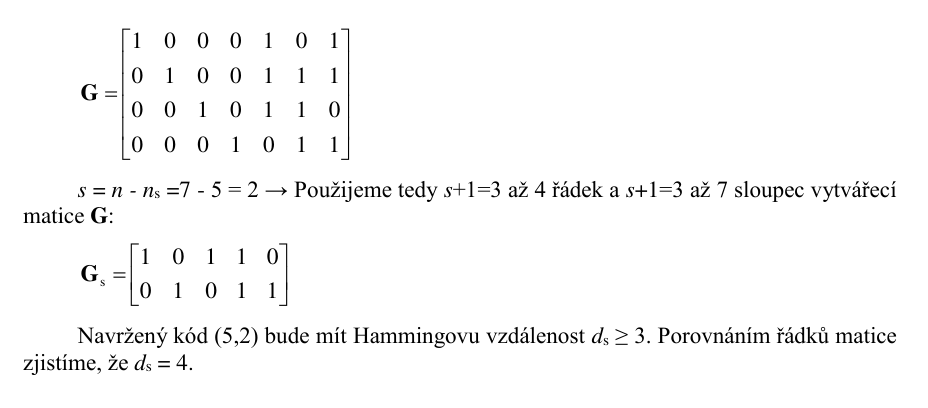
\includegraphics[width=16cm]{images/9_zkrac_priklad.png}

\subsection{Co specifikuje Hammingova hranice?}
\begin{itemize}
    \item Udává, kolik chyb je kód schopen opravit
    \item Počet syndromů, $2^{n-k}$ musí být větší nebo roven počtu kombinací chyb:
    $$2^{n-k}\geq \sum_{e=0}^t \binom{n}{e}$$
\end{itemize}

\subsection{Co je to prokládaní a proč se používá? Jaké znáte metody prokládaní?}
Je to metoda, která umožňuje změnou pořadí prvků dosáhnout změnu typu chyb ze shlukových na nezávislé. V minulosti hlavně u přenosu televizního obrazu z důvodu veliké potřebné šířky pásma (blikání). Nejběžnější \textbf{metody} prokládání jsou: Konvoluční prokládání a blokové prokládání.

\subsection{Co je to prokládání a proč se používá?}
\begin{itemize}
    \item interleaving
    \item Změna pořadí prvků -> změna shlukových chyb na nezávislé
\end{itemize}
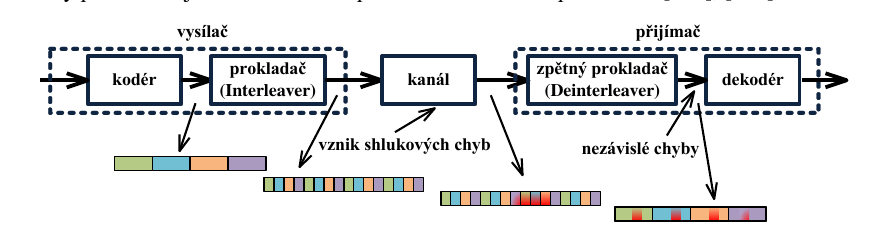
\includegraphics[width=16cm]{images/9_prokladani.png}

\subsection{Jaké znáte základní dvě metody prokládání?}
\begin{itemize}
    \item Blokové - do prokladače jdou bloky jako  řádku, z něj se čte po sloupcích
    \item konvoluční - trojúhelníkové pole zpožďovacích článků v prokladači a zpětném prokladači
    (každý další řádek má o 1 zpožďovací článek navíc, u zpětného naopak) \\
    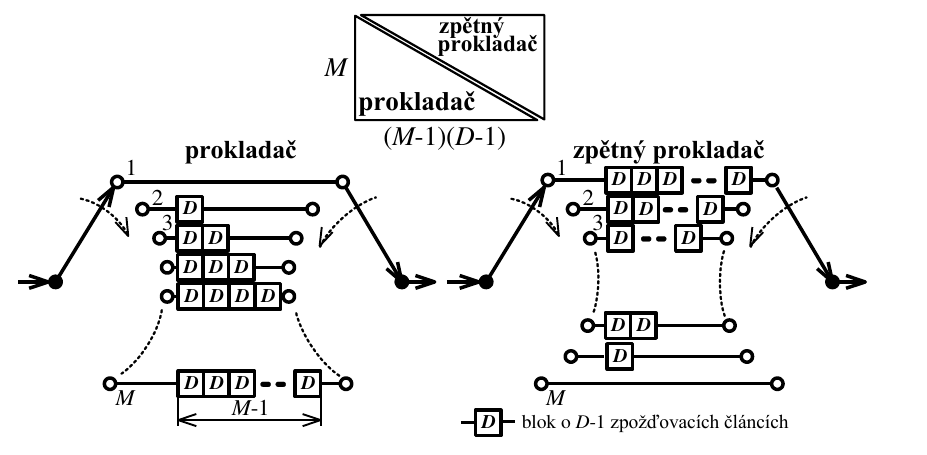
\includegraphics[width=16cm]{images/9_konvol_prokl.png}
\end{itemize}

\subsection{Co udává hloubka prokládání \textit{D}?}
Počet bloků účastnících se prokládání

\subsection{Co jsou to zřetězené kódy?}
\begin{itemize}
    \item výsledný zabezpečený datový tok z prvního kodéru je následně ještě jednou zabezpečen dalším kódem
    \item  Metoda se často kombinuje s prokládáním. Pro dekódování se vyžívaná modifikovaná Viterbiho metoda.
\end{itemize}

\subsection{Jaké dva základní typy zřetězení existují a jak se označují?}
\begin{itemize}
    \item paralelní zřetězení (turbo kódy)
    \item sériové zřetězení - násobné kódy (product code)
\end{itemize}

\subsection{Která technika se často využívá při zřetězení kódů?}
\begin{itemize}
    \item Metoda zřetězení se často kombinuje s prokládáním. Pro dekódování se vyžívaná modifikovaná Viterbiho metoda.
\end{itemize}

\subsection{Stručně vysvětlete princip měkkého dekódování algoritmem SOVA.}
\begin{itemize}
    \item Podobný Viterbiho algoritmu, používá mřížový diagram
    \item Určuje maximální akumulovanou pravděpodobnost pro každý stav místo ceny cesty
    \item Používá se proměnná $L_i$, která: $L_i=1$, pokud se shoduje v obou bitech,
    $L_i=0$ pokud v 1, $L_i=-1$ pokud v žádném
    \item Postupuje se od konce, zjistí se tvrdý výstup
    \item Celková pravděpodobnost každého stavu je součet pravděpodobnosti okamžitého stavu a apriorní pravděpodobnost,
    $L=L_i+L_p$
    \item Jsou brány v potaz také nepřežívající cesty, z nich je počítá funkce Delta (rozdíl hodnot L pro cesty), 
    z nich se tvoří měkký výstup
    \item Rozhodnutí se mění, pokud se mění bity
    \item Hodnoty funkce Delta jsou měkkým výstupem, upraví se koeficientem spolehlivosti kanálu
    \item První dekodér získá systematická data, druhý kodér získá kódovou informaci, která se předá druhému 
    dekodéru a takto iterujeme, záleží na implementaci, nakonec je kladným hodnotám přiřazen bit 1, záporným 0
\end{itemize}

\clearpage
\section{Protichybové kódové systémy}
\subsection{Uveďte základní dvě skupiny protichybovýh kódu (PKS). Vysvětlete rozdíl mezi nimi.}
\begin{itemize}
    \item \textbf{PKS bez zpětné vazby} - Zabezpečení pomocí opravných protichybových kódů (\textbf{FEC}). Zabezpečení pomocí detekčních protichybových kódů bez zpětného kanálu (Všechny chybné přenesené zprávy jsou ztraceny). Zabezpečení pomocí protichybových kódů pracujících ve $smíšeném$, tj. opravném i detekčním režimu (Většina chybné přenesených zpráv je opravena, část chybné přenesených zpráv je ztracena.)
    \item \textbf{PKS se zpětnou vazbou} - Zabezpečení pomocí detekčních  protichybových kódů s opakováním chybného přenosu (\textbf{ARQ}) (snížení propustnosti). Smíšené zabezpečení pomocí protichybových kódů pracujících v opravném i detekčním režimu - většina chybně přenesených zpráv je opravena (\textbf{FEC}), pro neopravitelné zprávy je využit mechanizmus ARQ.
\end{itemize}

\subsection{Uveďte a stručně popište základní typy ARQ systémů}
Chyba je opravena novým bezchybným přenosem. Při tom všechny předcházející přenosy s chybou jsou považovány za nepoužitelné
\begin{itemize}
    \item \textbf{Jednobloková ARQ} - Vysílač vyšle vždy pouze jeden blok, a pak se přenos přeruší až do doby, než přijde zpětným kanálem potvrzovací zpráva o správnosti přenosu. Opakovaní přenosu/pokračování
    \item \textbf{Skupinové ARQ} - Vysílač vyšle vždy skupinu bloků, každý blok nezávisle zabezpečený detekčním kódem. Přijímač informuje zpětným kanálem vysílač o bezchybnosti celé skupiny.
    \item \textbf{Nepřerušované ARQ} - Vysílač vysílá bloky bez přerušení až do doby, kdy přijde zpětným kanálem zpráva o tom, že některý blok byl přijat s chybou. Reakce selektivní/neselektivní opakování.
\end{itemize}
\subsection{Rozdíl mezi ARQ a FEC, výhody a nevýhody.}
\textbf{FEC} + Většina chybně přenesených zpráv je opravena. - Část chybné (neopravitelné) přenesených zpráv je ztracena. 

\textbf{ARQ} + Výhodou je použití detekčních kódů, jejichž nadbytečnost je nižší než u kódu opravných. - Významnou nevýhodou je snížení propustnosti z důvodu čekání na potvrzovací zprávy. - přenosový systém schopen realizovat některou podobu zpětného kanálu.

\subsection{Co udává propustnost systému a efektivní informační rychlost?}
\begin{itemize}
    \item Rozlišujeme propustnosti:
    \begin{itemize}
        \item absolutní ($PR$) - poměr úspěšně přenesených datových jednotek a časového intervalu 
        (totožné s efektivní informační rychlostí)
        \item relativní ($PR_r$) - poměr úspěšně přenesených jednotek za časový interval k maximálnímu
        možnému přenositelnému množství datových jednotek za tento interval
        \item Datové jednotky mohou být bity, znaky, bloky, zprávy
    \end{itemize}
    \item efektivní informační rychlost - poměr úspěšně přenesených datových jednotek a časového intervalu 
\end{itemize}

\subsection{Jaký vztah je mezi kódovým poměrem a efektivní informační rychlost v ARQ systémech a
v FEC systémech.}
\begin{itemize}
    \item ARQ: $v_{ef}=PRB_r\cdot R$, kde $v_{ef}$ je efektivní informační rychlost, $PRB_r$ je relativní propustnost
    a $R$ je kódový poměr, $R=\frac{k}{n}$, kde $k$ je počet informačních bitů a $n$ je počet všech bitů
    \item FEC: $v_ef=R$, protože $PRB_r$ je díky opravám chyb rovno jedné
\end{itemize}

\subsection{Srovnejte ARQ a FEC protichybové systémy.}
\subsubsection{ARQ}
\begin{itemize}
    \item \textbf{A}utomatic \textbf{R}epeat Re\textbf{q}uest
    \item Používá detekční kódy
    \item Při detekci chyby vyšle data znovu
    \item Efektivní informační rychlost závisí na chybovosti kanálu, kódovém poměru a algoritmu ARQ 
    (Při Stop\&Wait je propustnost nízká vždy, při GoBackN je propustnost nízká u kanálu  s vysokou chybovostí.
    ARQ SelectiveRepeat je vhodné jen na zařízení s dostatečně velkou vyrovnávací pamětí)
    \item Vyžaduje zpětný kanál, kterým se vysílač dozví o nutosti opakování nebo potvrzení přijetí
\end{itemize}
\subsubsection{FEC}
\begin{itemize}
    \item \textbf{F}orward \textbf{E}rror \textbf{C}orrection
    \item Používá korekční kódy
    \item Při výskytu chyby rovnou opraví
    \item Efektivní informační rychlost závisí na kódovém poměru 
    (ale musí být vhodně zvolen, aby eliminoval chybovost kanálu)
    \item Nevyžaduje zpětný kanál
\end{itemize}

\subsection{Uveďte výhody a nevýhody systému se smíšeným zabezpečením HCS}
\begin{itemize}
    \item \textbf{H}ybrid \textbf{C}ode \textbf{S}ecurity
    \item Výhody:
    \begin{itemize}
        \item Může používat jediný kód s korekčními i detekčními vlastnostmi
        \item V případě detekce chyby je možné vyžádat si korekční doplněk (bity potřebné k úpravě kódu na korekční)
    \end{itemize}
    \item Nevýhody:
    \begin{itemize}
        \item Oproti korekčnímu režimu mívají kódy ve smíšeném režimu menší realizační zisk
        \item Pokud chceme použít kaskádově zapojené detekční a korekční kódy, musíme je vhodně volit, ať se vzájemně
        neovlivňují
    \end{itemize}
\end{itemize}
\clearpage
\section{Modemy v systémech datové komunikace}
\subsection{Jaké jsou základní části modemu? Odůvodněte jejich použití.}

\subsection{Na jaké základní dvě skupiny dle použitého kmitočtového pásma lze rozdělit měniče
signálu? Vysvětlete pojmy linkový kód, klíčování a modulace, přidružte je výše
dotazovaným skupinám.}

\subsection{Co je to skrambler a k čemu slouží?}

\subsection{K čemu slouží linkové kódy? Jaké jsou základní důvody jejich použití? Uveďte příklady
linkových kódů a technologie, kde se využívají.}

\subsection{Uveďte a popište základní typy klíčování? Uveďte vícestavové klíčovací metody.}
Pozn. \textbf{Skrambler} umožňuje odstranění periodicit a dlouhých sekvencí stejných prvků. Přenos v \textbf{základním pásmu} se realizuje pomocí \textbf{linkových kódů}. Linkové kódování definuje realizace signálových prvků tak, aby byla zejména potlačena stejnosměrná složka.
\begin{itemize}
    \item Při přenosu dat v přeloženém pásmu se používá \textbf{modulační} proces, který nazýváme \textbf{klíčování}
    \item Základní typy klíčování: Amplitudové klíčování (ASK), Fázové klíčování (PSK), Kmitočtové klíčování (FSK).
    \item \textbf{Amplitudové klíčování} lze realizovat pomocí násobičky. Vynásobením nosného signálu datového signálu vznikne amplitudově klíčovaný signál. 
    \item \textbf{Kmitočtové klíčování} lze realizovat přepínáním dvojice oscilátorů nosných signálů s užitím násobičky.
    \item \textbf{PSK} je dvojstavové fázové klíčování. Klíčování je opět realizováno pomocí násobičky, na kterou je přivedena nosná a bipolární datový signál .
\end{itemize}
Čtyřstavové fázové klíčování (QPSK), Osmistavové fázové klíčování (8 - PSK)

\subsection{Vysvětlete princip QAM modulace. O jaký typ klíčování se jedná? Co je to IQ modulátor, zakreslete obrázek. Co je to konstelační diagram? }
\begin{itemize}
    \item V bloku OSMS je datový tok rozdělen na dva o shodné přenosové rychlosti.  Vzniklá dvojice signálů je vstupem IQ modulátoru. Číslice před zkratkou QAM uvádí počet stavů.
    \item Kvadraturní amplitudová modulace (QAM) reprezentuje vícestavové kombinované ASK-PSK klíčování.
    \item Protože jeden signál je ve fázi a druhý o pí/2 posunut, označují se tato dvojice jako \textbf{IQ modulátor}.
    
    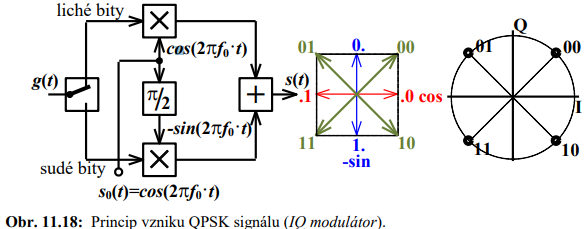
\includegraphics[]{images/image1.png}
    
    \item Fázové klíčování, ale především QAM, se zobrazují s pomocí tzv. \textbf{Konstelačního diagramu}. Diagram uvádí v IQ rovině přiřazení binárních kombinací fázorům nosného signálu.
\end{itemize}

\subsection{Modulace v pojetí protichybového sytému. Co je to eukleidovská vzdálenost? Popište
TCM modulaci?}

\subsection{Vysvětlete princip vícetónových modulací DMT/OFDM. Nakreslete obrázek realizace.}
\begin{itemize}
    \item Hledání metod dalšího zefektivnění datového přenosu vedlo k vícetónovým modulačním metodám.
    \item Můžeme se setkat s \textbf{Diskrétní vícetónovou modulací DMT}, která se uplatňuje zejména na telefonních přípojkách v ADSL a VDSL  
    \item a \textbf{Ortogonálním kmitočtově děleným multiplexem OFDM}, který se uplatňuje na sdílených médiích v technologiích PLC, WLAN, DVB-T. 
    \item Výsledkem aplikace IFFT je 2N komplexních hodnot. Ty jsou vstupem IQ modulátoru, který může být realizován s ohledem na cílové kmitočtové pásmo číslicově nebo analogově
\end{itemize}
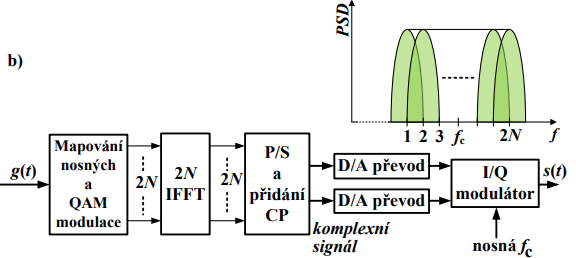
\includegraphics[]{images/image.png}
    
\subsection{Vysvětlete problematiku korekce přenosových charakteristik. Jaké typy ekvalizérů znáte?}

\subsection{Vysvětlete možnosti realizace duplexního přenosu. Co je to vidlice? Vysvětlete princip
vzniku a potlačení ozvěnového signálu.}

\clearpage
\section{Základy šifrování}
\subsection{Vysvětlete pojmy kryptografie, kryptoanalýza a kryptologie. Jaké hlavní úkoly plní kryptografické systémy? Jaké základní typy operací používá?}
\begin{itemize}
    \item \textbf{Kryptografie} - Věda zabývající se problematikou navrhování šifrovacích metod.
    \item \textbf{Kryptoanalýza} - Věda zabývající se luštěním zašifrovaných textů bez znalosti tajného klíče (prolamování)
    \item \textbf{Kryptologie} - Věda zabývající se studiem problematiky šifrování a dešifrování
    \item \textbf{Důvěrnost} - Utajení informace před neoprávněnými uživatelem. \textbf{Autentičnost} - Příjemce má možnost zjistit původ zprávy. \textbf{Integrita} - Kontrola zprávy, zda nebyla během přenosu modifikována. \textbf{Nepopiratelnost} - Odesílatel by neměl mít možnost popřít autorství zprávy.
    \item Jednoduché aritmetické operace (operace součtu modulo dvě), Substituce (znak původní zprávy se nahradí definovaným způsobem jiným znakem), Permutace (změní se definovaným způsobem pořadí znaků ve zprávě)
\end{itemize}

\subsection{Zakreslete a popište schéma kryptografického systému.}

\subsection{Jaké jsou základní pravidla kryptografie?}

\subsection{Uveďte základní typy operací využívaných v kryptografii?}

\subsection{Symetrické a asymetrické kryptosystémy (varianty), výhody + příklad použití}
\textbf{Symetrické}
\begin{itemize}
    \item Systémy s tajným, jediným klíčem
    \item Používají se v případech dvoubodového spoje
    \item\textbf{  - }Problém distribuce klíče (DH), Nelze prokázat totožnost autora zašifrovaných dat
    \item\textbf{ + }Velmi rychlé algoritmy, šifrování velkých objemů dat.
    \item Caeserova šifra, Vigenérova šifra (substituce), DES, AES
\end{itemize}
\textbf{Asymetrické}
\begin{itemize}
    \item Systémy s veřejným klíčem, klíče jsou navzájem různé a výpočet Kv → Ks je prakticky nerealizovatelný
    \item Jeden klíč je veřejný (zajištění důvěrnosti a integrity)  a druhý tajný (zajištění autentičnost dat)
    \item Využití problému faktorizace velkých čísel, diskrétního logaritmu, eliptických křivek
    \item  K podepisování zpráv a k distribuci klíčů pro symetrické kryptosystémy
    \item\textbf{ - }Pomalejší, zapotřebí infrastruktura veřejných klíčů 
    \item\textbf{ + }Umožňuje zajištění důvěrnosti, integrity a autentičnosti dat 
    \item RSA, DH
\end{itemize}

\subsection{Stručně popište kryptosystémy DES a AES.}

\subsection{Stručně popište metodu RSA. Na čem je založena její bezpečnost?}

\subsection{Stručně popište metodu Diffie-Hellman a uveďte příklady využití.}

\subsection{Co je to digitální otisk (heš). Vysvětlete využití.}

\end{document}
